\documentclass[11pt]{article}

\usepackage{microtype}
\usepackage{amsmath}
\usepackage{xcolor}
\usepackage{graphicx}
\usepackage{enumitem}


\setlength{\parindent}{0cm}
\renewcommand\thesubsection{\alph{subsection})}

\title{\textbf{Assignment 2\\}Search Algorithms}
\author{Malik Al-hallak 90020\\
		Sebastian Utzig 100059\\
		Clemens Wegener 91268}
\date{}
\begin{document}

\maketitle

\section{Matchsticks}
\subsection{}
The problem-reduction graph is better suited, since the problem is serializable and the problem-reduction graph can take advantage of that. This minimizes the size of the graph and can represent the problem for any initial count of matchsticks, without altering the representation.

\subsection{}
The statspace can be described by two variables: S=(\texttt{number\_of\_matchsticks, whos\_turn}).
Where \texttt{number\_of\_matchsticks} is the count of sticks on the table and \texttt{whos\_turn} is either "opponent" or "player". The operators are \texttt{OP={-1,-2,-3}} denoting the take away of the respective count of matchsticks from the table.

\subsection{}
A solved leave node is the state \texttt{(1, "opponent")}.

\subsection{}
A node can be seen as solved, when there is a path to a solved leaf node through at least one OR-connection and all AND-connections between the node and the leave node.

\subsection{}
For the player who takes the first turn: If the number of matchsticks is not a target number (i.e., when $\texttt{number\_of\_matchsticks} \% 4 \neq 1$), then the distance to the next target-number is $\leq3$ . So by taking away at maximum three matchsticks, the player is able to produce the target-number for the opponent. Since the opponet always as  target number of matchsticks on the table, he is not able to produce a target number of matchsticks for the player (since the distance is 4).
The smallest target-number is 1, so the player who takes the first turn will win.

However, if the player who takes the first turn encounters a target number of matchsticks on the table, the distance to the next target number is 4 and there is always a strategy for the opponent to produce the target number again and again for the players next turn. So the player who takes the frirst turn will loose. 

\subsection{}
Please find the python code attached in the file \texttt{matchsticks.py}.

\section{Serializability}
The 8 queens problem is not serializable. There can't be a subproblem, that doesn't compromise another subproblem, because the attack radius of the queens reach into the area of other potential subproblems.

\section{Depth-first search in a graph}
\subsection{}
By using two different lists where we store already expanded nodes (CLOSED) and to be visited successors (OPEN) multiple expansions of a single node are avoided. Therefor we stack the unexplored nodes in a LIFO manner and move the explored into the CLOSED list in order to traverse the graph in depth-first.


\subsection{}
Simply checking whether a to be expanded node is already in the CLOSED list could easily avoid it's second expansion. However, it may be difficult to remember the first expansion if we cleaned up the CLOSED list in between. In this case we could not detect a cycle reaching into an already visited and solved branch.


\subsection{}
We can escape the maze by simply solving a depth-first search problem with Trémaux's algorithm. Assuming we can mark the paths chosen on a junction once per run (and a second time if we have to go back) it is possible to find the solution path efficiently by choosing the path with the lowest mark number at each junction. Whenever we reach a marked junction and our path we came from is marked just once we go back. If a solution path exists all paths on this way will be marked just once. If not we will get back to the starting point. A path is always either unvisited, marked once or marked twice.



\section{Search Space}
The method \texttt{cleanup\_closed} removes nodes from the CLOSE list which are not part of the solution path. All dead end nodes fulfill this criterion, therefore the nodes \emph{k} and \emph{u} are deleted. Furthermore, all predecessors of the deleted dead end nodes which don't have successors on the OPEN list, and therefore cannot be part of the solution path, can be deleted. Node \emph{c} fulfills this and hence is deleted too.


\begin{figure}[ht]
	\centering
  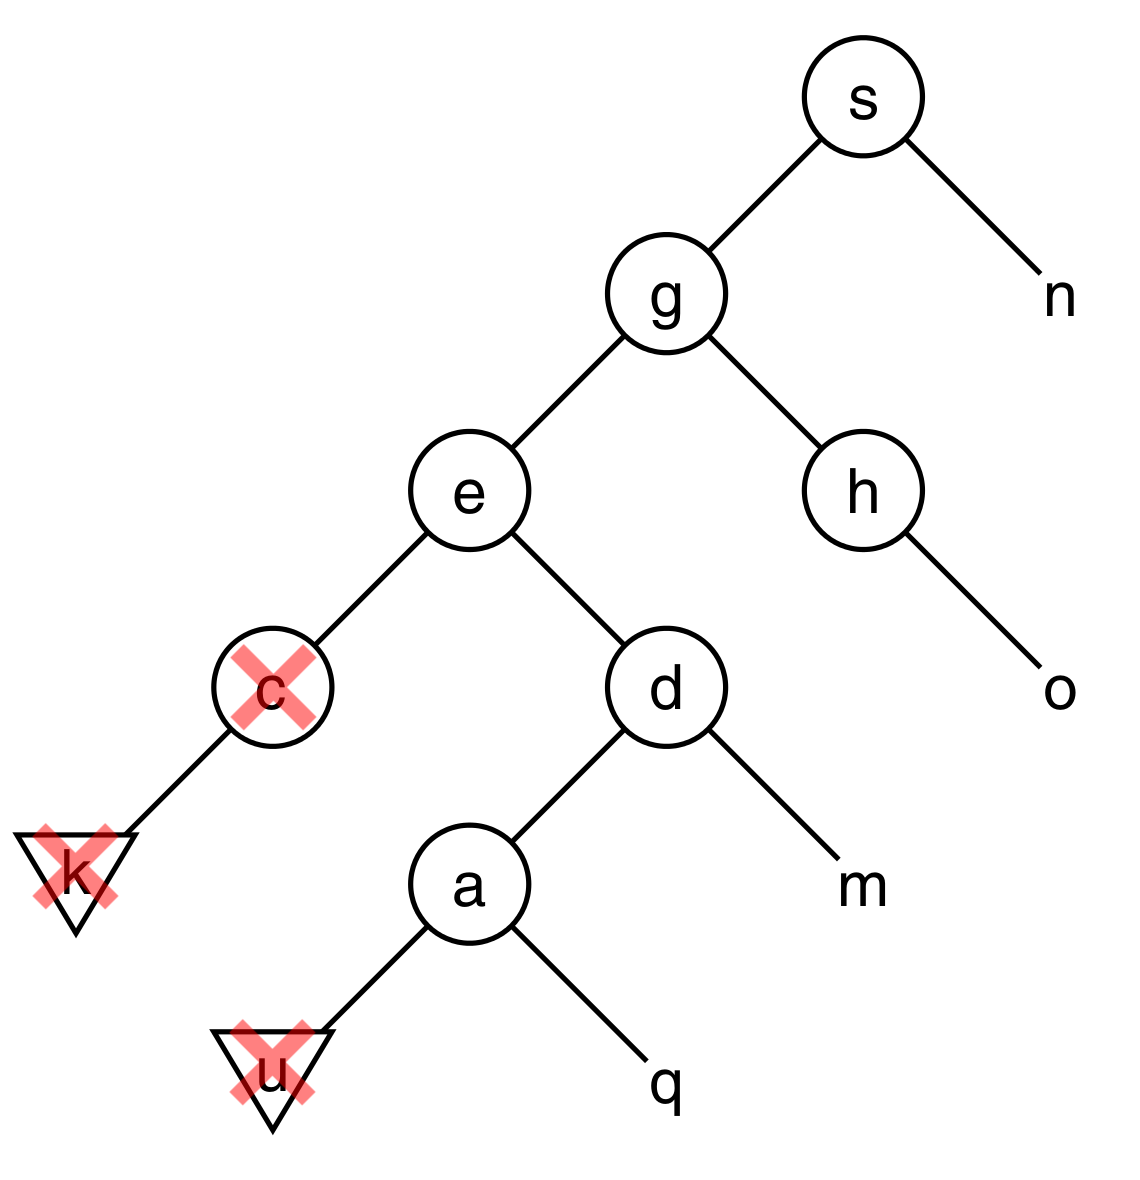
\includegraphics[width=0.5\textwidth]{./graph_7.png}
  \caption{Graph after \texttt{cleanup\_closed}}
	\label{fig2}
\end{figure}

\setcounter{section}{6}
\section{Hill-Climbing}

\begin{minipage}{0.5\textwidth}
	\subsection{}
	\begin{align*}
		n=s=0\\
		n_{opt}=s=0\\\\
		n_{opt}=2\\
		n_{opt}=3\\\\
		n_{opt}=4\\
		n_{opt}=6\\\\
		n_{opt}=7^*\\
		n_{opt}=8^*\\\\
		return\hspace{0.3cm}n_{opt}=8^*
	\end{align*}
\end{minipage}
\begin{minipage}{0.5\textwidth}
	\subsection{}
	\begin{align*}
		n=s=0\\
		n_{opt}=s=0\\\\
		n_{opt}=1\\
		n_{opt}=3\\\\
		n_{opt}=2\\
		n_{opt}=5\\\\
		n_{opt}=6\\\\\\
		return\hspace{0.3cm}Fail
	\end{align*}
\end{minipage}


\end{document}
